% arara: pdflatex
% arara: bibtex
% arara: pdflatex
% arara: pdflatex
% 
% Annual Cognitive Science Conference
% Sample LaTeX Paper -- Proceedings Format
% 

% Original : Ashwin Ram (ashwin@cc.gatech.edu)       04/01/1994
% Modified : Johanna Moore (jmoore@cs.pitt.edu)      03/17/1995
% Modified : David Noelle (noelle@ucsd.edu)          03/15/1996
% Modified : Pat Langley (langley@cs.stanford.edu)   01/26/1997
% Latex2e corrections by Ramin Charles Nakisa        01/28/1997 
% Modified : Tina Eliassi-Rad (eliassi@cs.wisc.edu)  01/31/1998
% Modified : Trisha Yannuzzi (trisha@ircs.upenn.edu) 12/28/1999 (in process)
% Modified : Mary Ellen Foster (M.E.Foster@ed.ac.uk) 12/11/2000
% Modified : Ken Forbus                              01/23/2004
% Modified : Eli M. Silk (esilk@pitt.edu)            05/24/2005
% Modified : Niels Taatgen (taatgen@cmu.edu)         10/24/2006
% Modified : David Noelle (dnoelle@ucmerced.edu)     11/19/2014

%% Change "letterpaper" in the following line to "a4paper" if you must.
 
\documentclass[10pt,letterpaper]{article}
 
\usepackage{hyperref}
\usepackage{cogsci}
\usepackage{pslatex}
\usepackage{amsfonts}
\usepackage{graphicx}
\usepackage{apacite}
\usepackage{color}
\usepackage{todonotes}
\usepackage{dsfont}
\usepackage{textcomp}
\usepackage{listings}

\definecolor{Red}{RGB}{255,0,0}
\newcommand{\red}[1]{\textcolor{Red}{#1}}

\newcommand{\jd}[1]{\green{$^*$}\marginpar{\footnotesize{JD: \green{#1}}}}

\newcommand{\subsubsubsection}[1]{{\em #1}}
\newcommand{\eref}[1]{(\ref{#1})}
\newcommand{\tableref}[1]{Table \ref{#1}}
\newcommand{\figref}[1]{Figure \ref{#1}}
\newcommand{\appref}[1]{Appendix \ref{#1}}
\newcommand{\sectionref}[1]{Section \ref{#1}}

\title{What do newspapers, watches, credit cards, and liquors bottles have in common? A computational exploration of question behavior.}
 
\author{{\large \bf Robert X.~D.~Hawkins, Noah D.~Goodman}}

\begin{document}

\maketitle

\begin{abstract}
What makes a question useful? What makes an answer appropriate? In this paper, we show that a recently proposed probabilistic model of question-answer behavior provides a unifying account of four separate effects from the psycholinguistics and pragmatics literature. For three of these effects, we formulate a pragmatic answerer who is  informative with respect to the questioner's underlying goals (or QUD), which are inferred given the context. These simple applications illustrate the role of the QUD in guiding answerer inference. In the final effect we model, the questioner's QUD affects the question they choose to ask; thus, our pragmatic answerer may use the question utterance itself as a signal to help infer the questioner's goals. 

\textbf{Keywords:} 
language understanding; pragmatics; Bayesian models; questions; answers
\end{abstract}

\section{Introduction}
\label{sec:intro}

% TODO:
% * think of other good discussion points

\begin{quote}
Q:``Are you gonna eat that?''\ \ A:``Go ahead.''
\end{quote}
In this (real life) example, Q strategically chooses a question that differs from her true interest, avoiding an impolite question, yet manages to signal to A what her interests are; A in turn reasons beyond the overt question and provides an answer that addresses Q's interests.
This subtle interplay raises two questions for formal models of language:
What makes a question useful? What makes an answer appropriate? 
%\red{RDH: I commented out a bunch here that was restating the abstract... Might put back in if we have enough space}
%In this paper, we present three progressively more sophisticated computational models of question-answer behavior.
%, which formalize and probe the way answerers infer intentions and the way questioners signal them. 
%We compare these models on the basis of a simulation of a classic question-answer phenomenon and two experiments in which participants must ask and answer questions in a communication game where we can experimentally manipulate the available questions and answers.
%We find that sophisticated pragmatic reasoning is needed to account for some of the data. This suggests that people are able to engage in such reasoning when it is beneficial: they can use questions to provide cues to the answerer about their interest, and can select answers that are informative about inferred interests.

%A:"can you pass he salt?"
%B:"yes (i am able)."



%Suppose your friend asks you, ``Who is coming to the concert tonight?'' How do you respond? You certainly don't need to give the full list of attendees -- most of whom you do not know -- even though they would all technically be valid answers. Instead, you might only mention the set of \emph{mutual acquaintances} you know are planning to come, assuming that your friend doesn't care about the rest of the crowd. Now, imagine a different scenario. Suppose that you're waiting in line at the box office and want to find out whether your acquaintances had tickets as well. What question would you ask to the person in the ticket booth? If you asked, ``Who is coming to the concert tonight?''  you would likely get a quizzical look and an answer like ``A lot of people, why?'' because the person at the booth does not know your friends or your reason for asking the question. Instead, you might have to directly ask about your friends. Whether you're asking or answering questions, you must engage in some reasoning about the other person's intentions and knowledge. 
%
%Since both questioners and answerers appear to be acutely sensitive to one another's intentions and knowledge, what makes a question useful? What makes an answer to a question useful? In this paper, we present three progressively more sophisticated computational models of question-answer behavior, which formalize and probe this deep interaction between the way answerers infer intentions and the way questioners signal them. We compare these models on the basis of two simulations of classic question-answer phenomena and one experiment in which participants must ask and answer questions given a fixed set of goals. We find that a sophisticated pragmatic answerer is needed to account for the data, and close by proposing that the purpose of questions in dialogue is to provide cues to the answerer about the questioner's goals and intentions.

%\red{RDH: Want to motivate RSA a bit more? We've got some space!}
Recent work on Rational Speech Act (RSA) models \cite{frank2012, GoodmanStuhlmuller13_KnowledgeImplicature} has mathematically formalized pragmatic language understanding as a form of recursive Bayesian inference, where listeners reason about speakers who choose utterances that maximize information gained by an imagined listener.
%a particular utility function (dependent on the listener's expected information gain). 
In this paper we extend the RSA framework to address simple question-answer dialogs.
%asking questions and giving answerers. 
The immediate challenge in doing so is that the speaker utility in RSA is based on direct information provided by an utterance---since questions don't provide direct information, we must say what utility they do have. 

We suggest, following \citeA{VanRooy03_QuestioningDecisionProblems}, that the value of a question is the extent to which it can be expected to elicit information relevant to the questioner later in the dialogue. 
More specifically, for the questioner, the value of a question is the expected information gained about her interests, given the set of likely answers it may provoke. 
This diverges from regular RSA in that the value of a question depends on information gained by the speaker (rather than listener), and that this information comes later in the (very short) conversation.

To fully specify this questioner we need a model of the answerer, which can serve as both the model assumed by a questioner, and as a model of answer behavior itself. As in previous RSA models, we construct a sequence of progressively more sophisticated answerers. At the most na\"ive level, the answerer provides a literal answer to the question (without attempting to be informative); at the most sophisticated level, a pragmatic answerer infers the most likely true interests of the questioner, and then informatively addresses those interests. The latter model extends RSA to reason about the topic of conversation, as proposed by \citeA{kao2014nonliteral} to explain hyperbole; it goes beyond previous work by using the explicit question as a (potentially indirect) cue to this topic. 

%In particular, we compare a pragmatic answerer making inferences about the questioner's goals to two simpler models: one that takes into account only that an answerer wants to be maximally informative with respect to the explicit question asked (without inferring the questioner's underlying decision problem) and one that provides a literal answer to the question (without attempting to be maximally informative).  

The rest of this paper is structured as follows. First, we lay out the details of our question-answer model and contrast our approach with some related models (notably the decision-theoretic approach proposed by \citeauthor{VanRooy03_QuestioningDecisionProblems}, 2003). We then proceed to introduce the four scenarios we wish to model and show that the same pragmatic answerer model can qualitatively account for all of the effects observed in these scenarios.
%accommodate  some classic psycholinguistic phenomena .
%We find that the most sophisticated, pragmatic models best account for human performance.
%derive predictions for a  of experiments using a novel guessing-game task, and compare these predictions to human performance. 
%In one phase of the task, we require participants to ask a question (from a fixed set of possible questions), given a decision problem. In the second phase, we require participants to give an answer (from a fixed set of possible answers) to a question (from a fixed set of possible questions). 
We close with a brief discussion of future directions.
%These models and data, combined with the psycholinguistic data above, seeks to place question-answer behavior in the larger class of social behavior governed by theory of mind.

\section{Background and Related Work}

How should a questioner choose between questions?
%
We start by assuming that the questioner aims to \emph{learn information relevant to a private goal}.
%
In order to choose a question that results in useful information, the questioner reasons about how the answerer would respond, given different possible states of the world; she selects a question that results in an answer that tends to provide goal-relevant information.
%

% This is a divergence from previous RSA models, where agents choose utterances with the goal of imparting information about the state of the world.

More formally, suppose there is a set of world states $\mathcal{W}$, a set of possible goals $\mathcal{G}$, a set of possible questions $\mathcal{Q}$, and a set of possible answers $\mathcal{A}$.
These sets are taken to be in common ground between the questioner and the answerer.
An informational goal $g \in \mathcal{G}$ is a projection function that maps a world state to a particular feature or set of features that the questioner cares about; this is similar to the notion of a question-under-discussion \cite{Roberts96_InformationStructureDiscourse}.
We will use the notation $P_{g}(w)$ to indicate the probability $\hat{P}(g(w))$ of the $g$-relevant aspect of $w$ under the projected distribution 
$\hat{P}(v) = \int_{\mathcal{W}} \delta_{v=g(w)}P(w)dw$.
% Each of these projections corresponds to a different utility function, in a decision-theoretic formulation.
%In order to learn information about their private goal $g$, the questioner reasons about how an internal model of an answerer would respond given some true world.

\newcommand{\KL}[2]{\ensuremath{D_{KL}({#1}\, \| \, {#2})}}
\newcommand{\E}[2]{\ensuremath{\mathbb{E}_{#1}\left [#2 \right]}}

The \textbf{questioner} takes a goal $g \in \mathcal{G}$ as input and returns a distribution over questions $q \in \mathcal{Q}$:
%
$$ 
P(q|g) \propto e^{\E{P(w^*)}{\KL{P_g(w|q, w^*)}{P_g(w)}} - C(q)} 
$$
%
It trades off the cost of asking a question, $C(q)$, and expected information gain. The cost likely depends on question length, among other factors. Information gain is measured as the Kullback-Leibler divergence between the prior distribution over $g$-relevant worlds, $P_g(w)$, and the posterior distribution one would expect after asking a question $q$ whose answer reflected true world state $w^*$:
%
$$ P_g(w|q, w^*) = \sum_{a \in \mathcal{A}} P_g(w |q, a) P(a| q, w^*)$$
%
%This conditional distribution reflects the fact that the answerer (who knows the true world state $w$) may behave noisily, have a limited set of possible answers, or other limitations.
%to questioner (who is inferring a world state $w^*$) is affected by stochastic answerer behavior and a limited set of possible answers. 
This distribution has two components: 
First, it depends on $P(a | q, w^*)$, a model of the answerer which we will explore shortly.
Second, it depends on (the goal projection of) $P(w | q, a)$, an `interpreter' that specifies the likelihood assigned to different worlds given question and answer pairs.

To define the interpreter function, which all agents use to compute the literal interpretation of a question-answer pair, we must assign questions a semantic meaning.
We assume that a question is an informational goal that projects from worlds to the answer set $\mathcal{A}$.
This is equivalent to the more common partition semantics of \citeA{GroenendijkStokhof84_SemanticsOfQuestions}, as can be seen by considering the pre-image of such a projection; an answer picks out an element of the partition via $q^{-1}(a)$.
%For the purposes of this paper, we will use Groenendijk \& Stokhof semantics \citeyear{GroenendijkStokhof84_SemanticsOfQuestions}, where a question induces a partition $\mathcal{P}_q$ over the space of possible world and each cell of this partition is an equivalence class corresponding to a different answer. An answer, then, selects a cell of this partition, denoted by $\mathcal{P}_q(a)$, which is a set.
The \textbf{interpreter} constrains the prior on worlds to the subset of its support that is consistent with the semantics of a question-answer pair\footnote{We should also have a semantic evaluation function that maps an answer utterance to its value in $\mathcal{A}$. For clarity we assume this is a trivial mapping and suppress it.}:
%
$$P(w | q, a) \propto P(w) \delta_{q(w)=a}$$

We next describe two different answerer models; the questioner could assume any one of them, leading to two corresponding versions of the questioner model.
All answerers take a question $q \in \mathcal{Q}$ and a true world state $w^* \in \mathcal{W}$ as input and return a distribution over answers $a \in \mathcal{A}$.
%
The \textbf{literal answerer} simply chooses answers by trading off prior answer probability  and how well a question-answer pair conveys the true state of the world to an interpreter:
%
$$P(a | q,w^*) \propto P(a) P(w^* | q, a) $$
%
For a fixed question, this is equivalent to the speaker in previous RSA models. The question enters only in specifying the literal meaning of an answer.
%

The \textbf{pragmatic answerer} also evaluates answers with respect to how well they address the informational goal, but doesn't take the question's explicit meaning at face value. Instead, the pragmatic answerer reasons about which goals $g$ are likely given that a question $q$ was asked, and chooses answers that are good on average:
%% FIXME: restrict to truthful answers
%
$$
P(a | q, w^*) \propto p(a) \sum_{g \in \mathcal{G}} P(g|q) P_g(w^*|q, a)
$$
Reasoning backwards from questions to goals is a simple Bayesian inversion of the (explicit) questioner using a prior on goals:
$$
P(g|q) \propto P(q|g)P(g)
$$

For all of the questioner and answerer models, we can vary how strongly optimizing they are---that is, to what extent they are sampling from the distributions defined above, and to what extent they deterministically choose the most likely element. For any such distribution over utterances, we introduce an optimality parameter $\alpha$ and transform it by $ P'(x) \propto P(x)^{\alpha} $.
%

This concludes our specification of the model space, giving a set of two answerers and two corresponding questioners that reason about them. We have implemented these models in WebPPL, a probabilistic programming language \cite{GoodmanStuhlmuller14_DIPPL}, and runnable code for all reported simulations will be available online at \url{http://hawkrobe.github.io/Q_and_A/}. The model predictions shown throughout the rest of the paper are computed using this implementation.

This Bayesian account of question and answer behavior bears some resemblance to recent decision theoretic or game theoretic accounts in linguistics. These theories were a response to early work on question and answer semantics, which focused on the notion of informativeness. In Groenendijk \& Stokhof's \citeyear{GroenendijkStokhof84_SemanticsOfQuestions} theory of question and answer semantics, asking a question induces a partition over the space of possible worlds, where each cell of the partition corresponds to a possible answer. An answer, then, consists of eliminating cells in this partition, and the most useful answers are those that eliminate all relevant alternatives to the true world. However, as van Rooy \cite{VanRooy03_QuestioningDecisionProblems} and others \cite{Ginzburg95_ResolvingQuestions} have pointed out, this predicts that \emph{wh}-questions like ``Where can I buy an Italian newspaper?'' can only be fully resolved by exhaustively mentioning whether or not such a newspaper can be bought at each possible location. Clearly, this is not the case: a single nearby location would suffice. These theories also cannot account for  contextual variation in what counts as a useful answer, such as identification questions like ``who is X?'' \cite{BoerLycan75_KnowingWho}, and to questions like ``where are you?'' that permit answers at many levels of abstraction \cite{Potts12_CardsDialogueCorpus}. 

More recent theories have tried to fix these problems by introducing some consideration of the questioner's goals. van Rooy \citeyear{VanRooy03_QuestioningDecisionProblems}, for instance, formalizes these goals as a decision problem faced by the questioner. A useful answer under this decision theoretic account is one that maximizes the expected value of the questioner's decision problem. A useful question is one that induces a sufficiently fine-grained partition, optimally distinguishing the worlds relevant to the decision problem. While this framework elegantly accounts for the context-dependence and relevance-maximization of question and answer behavior, it assumes that the questioner's decision problem is known \emph{a priori} by the answerer. If this were the case, the act of asking questions would seem irrelevant: why wouldn't the answerer directly tell the questioner which action to take? Nevertheless, while empirical work has almost exclusively focused on \emph{answerer} behavior, van Rooy's approach suggests that the question itself is important in prompting a relevant answer. Our model is an effort to expand on this core idea in a probabilistic framework that also provides an inferential mechanism for the answerer to \emph{infer} the `decision problem' instead of assuming it.
 
\section{Four case studies}

\subsection{Clark (1979), Experiment 4}

First, we show that our model can provide different---sometimes over- or under-informative---answers to the same explicit question, depending on context. For this illustration, we model the whiskey-pricing study presented in the Introduction \cite{Clark79_IndirectSpeechActs}. Recall that liquor merchants were more likely to give over-informative answers (specifying exact price) to the question ``Does a fifth of Jim Beam cost more than \$5?'' in the uninformative context (``I want to buy some bourbon'') than in the five dollar context (``I've got \$5 to spend'').

Our world state is simply the whiskey's price (\$1, \$2, \dots, \$10). There are two possible goals: learning the price of whiskey and learning whether the price is greater than \$5. The set of answers includes exact prices as well as ``yes'' and ``no'', with lower cost for ``yes'' and ``no'' than the price statements. We model the context sentence as affecting the questioner's goal prior. When the context is ``I'd like to buy some whiskey,'' we assume that the the two goals are equally likely. When it is ``I only have \$5 to spend,'' we assume that it is 9:1 in favor of learning whether the price is greater than \$5.

\subsubsection{Results} When the question is ``Does Jim Beam cost more than \$5?'', the correct Boolean answer is  the most probable choice (at probability $.44$ and $.49$). Critically, there is a context-dependence for answers to this question: when prefaced with ``I'd like to buy some whiskey.'', the correct exact price answer is favored more strongly (at probability $.18$) than when the context is ``I only have \$5 to spend.'' (probability $.11$). By contrast, the literal and explicit answerers (which have no natural way to account for context) do not make differential predictions in the two situations. The literal model predicts that the answerer is equally likely to say the true Boolean answer and the true numerical answer, and the explicit model predicts that the answerer will always give the true Boolean answer, since it is the explicit question being asked. This suggests that our pragmatic \emph{answerer} is consistent with human behavior in psychologically interesting situations, passing a first, qualitative, test. 

\subsection{Groenendijk and Stokhof (1984)}

For a slightly more complex example, we consider the classic puzzle of \emph{mention-some} and \emph{mention-all} readings of wh-questions  \cite{GroenendijkStokhof84_SemanticsOfQuestions,SchulzVanRooij06_ExhaustiveInterpretation}. Some questions, like ``Who is coming to dinner tonight?'' are intended to elicit an exhaustive list of the entities that are answers. For other questions, like ``Where can I find a bathroom in this building?'', a single answer would be sufficient. 

The question ``Where can one buy an Italian newspaper?'' can intuitively be ambiguous between these meanings depending on who is asking: if it is a tourist, they probably just want to know the nearest place, but if it is a businessperson trying to build a newspaper distribution network in town, they likely want the whole list. The puzzle is determining how the same question can take on different semantics in different contexts: according to our account, this happens via an inference about the questioner's underlying goal.

Our world state is an object consisting of four cafes in town. Each cafe is assigned two properties: its distance from the speaker and whether or not it sells Italian newspapers. There are two possible goals: learning the identity of the \emph{nearest} cafe selling a newspaper and learning the identity of \emph{all} cafes selling a newspaper. The set of answers includes all 16 combinations of different cafes (e.g. ``cafe 1 and cafe 3'' or ``cafe 2, cafe 3, and cafe 4''), as well as the answer ``none''. 

The prior over answer utterances is constructed as follows: there is a 10\% chance of saying ``none,'' . Otherwise, the agent selects one of the four cafes and terminates with probability .5. If the agent does not terminate, they pick another cafe from the list and continue until either terminating or running out of possible cafes. This naturally gives longer answers lower probability, reflecting their higher cost of utterance. We model the context sentence as affecting the questioner's goal prior: if they say ``I'm new here,'' there is a 9:1 chance that they are interested in the closest location with a newspaper; if they say ``I'm a businessperson\dots,'' there is a 9:1 chance that they are interested in all of the newspaper locations. 

\subsubsection{Results}

For concreteness, we set the world to be the following :

\begin{lstlisting}
world = {'cafe1' : [3, false],
         'cafe2' : [1, true],
         'cafe3' : [3, true],
         'cafe4' : [3, true]}
\end{lstlisting}
and enumerated over all model executions for both contexts. We find that the highest probability response given the ``I'm new here'' context is the single location ``cafe2,'' with probability 0.56. Given the ``I'm a businessperson\dots'' context, however, the highest probability response is the conjunction ``cafe2 and cafe3 and cafe4,'' with probability 0.82. Note that cafe 1 was not assigned any probability in either context because it did not sell Italian newspapers (demonstrating that the pragmatic answerer will not lie), and that the nearest cafe was given precedence in the ``tourist'' context. 

The literal and explicit answerers, as in the Clark scenario, do not have the means of making inferences about the questioner's underlying goals. Thus, both models incorrectly predicted that the context would not affect the preferred response. The literal answerer predicted that all combinations of cafes 2, 3, and 4 would be given in proportion to their prior likelihood (with no special preference given to the closest one). The explicit answerer predicted that cafe2 would be preferred in all contexts.     Crucially, the only difference between our model of this scenario and the Clark scenario is the set of QUDs, the structure of the world, and the meanings of the answers. The questioner and answerer functions stayed exactly the same.

\subsection{Gibbs Jr. \& Bryant (2008): Experiment 3}

It has been shown in previous work that people typically round their answers to the nearest 5 or 10 minute interval when asked `Do you have the time?'', even when they're wearing a digital watch \cite{DerHenstCarlesSperber02_RelevanceTellingTime}.  \citeA{GibbsBryant08_OptimalRelevance} replicated this result, and then performed a follow-up study where they preceded their question by the context ``I have a meeting at 4:00.'' They found that the tendency to round times decreased as a function of the time remaining until the stated deadline: when people were asked at 3:40, they would say ``It's 3:45,'' but when people were asked at 3:53, they would make their response precise to the minute. They explain this result by appealing to the questioner's goals: while an approximate time is sufficiently informative with respect to most goals, a questioner who is running late to an appointment may have the goal of judging whether to rush, in which case a precise time is needed. 
  \begin{figure*}[t!]
\begin{center}
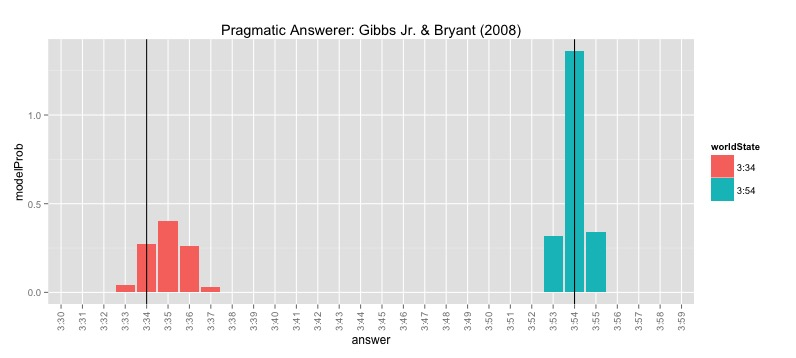
\includegraphics[scale = .5]{timeExpResults.jpeg}
\end{center}
\vspace{-.25cm}
\caption{Results for our computational experiments replicating Gibbs Jr. and Bryant (2008). Vertical lines represent the true world state.}
\label{fig:timeExperimentResults}
\end{figure*}
We take the world state to be the true current time. Unlike in the previous two scenarios, where there are only two QUDs and two contexts that make each QUD more or less likely, we now let there be a \emph{family of QUDs} and a fixed context stating the time of the appointment. This family of QUDs is parameterized by a threshold time, below which times are rounded to the nearest 5 minute increment and above which times are given exactly. For example, the QUD with the threshold set at 3:50 corresponds to a goal of wanting to learn the true time if it is higher than 3:50 and only caring about the approximate time below 3:50. The prior over thresholds ($\tau =$ 3:30, 3:35, \dots, 3:55), given a context sentence, weights each threshold by its distance to the appointment time, reflecting the intuition that the questioner will be more interested in the exact time as it approaches the appointment time.



 The set of answers is the set of times that could be given (e.g. 3:30, 3:31, \dots, 4:00), with uniform probability. Critically, the meaning of an answer is not exact: it introduces a factor in the ``interpreter'' component of the model, upweighting world states that are close to the answer utterance. In other words, we specify an ``approximate'' semantics for number references, which is necessary for rounded answers to be produced in the first place.
 


 \subsubsection{Results}
 
 To test the behavior of this model, we compare two simulations. In both, the context is ``I have an appointment at 4:00.'' In the first, the true world state is 3:34 (the `appointment far' condition); in the second, the true world state is 3:54 (the `appointment near' condition). Gibbs Jr. and Bryant \citeyear{GibbsBryant08_OptimalRelevance} found that the answerer is most likely to round to 3:35 in the `appointment far' condition, but most likely to give the exact time, 3:54, in the `appointment near' condition. Indeed, in the `appointment far' condition, the pragmatic questioner model, which infers which threshold is likely given the context and threshold, replies the rounded time `3:35' with probability 0.40 compared to the true time `3:34' with probability 0.27. In the `appointment near' condition, this pattern reverses: the pragmatic questioner model replies the rounded time `3:55' with probability 0.16 and the exact time `3:54' with probability 0.68 (see Figure \ref{fig:timeExperimentResults}).


\subsection{Clark (1979): Experiment 5}
  \begin{figure*}[t!]
  \begin{center}
\includegraphics[scale = .7]{creditCardPlot.jpeg}
\end{center}
\vspace{-.25cm}
\caption{Results for our computational experiments replicating Clark (1979), Experiment 4. M stands for the ``MasterCard'' answer, D stands for the ``Diner's Club'' answer, and $M+D$ stands for the answer mentioning both. Note that we give an over-informative answer to ``Do you accept any kinds of credit card?'' in the left panel, but a literal `yes'/`no' answer to ``Do you accept MasterCard?'' in the right panel.}
\label{fig:creditCardExperimentResults}
\end{figure*}
Our final scenario is a critical test for the questioner component of our model. Because the question space in the previous computational experiments only contained one element, the pragmatic answerers' inferences were entirely based on the context and the QUD prior. One of the most interesting and novel predictions of the RSA model, however, is that the questioner's choice of utterance itself should guide a pragmatic answerer's inferences about likely underlying goals. While there are few experimental results using questioner behavior as the \emph{dependent variable}, making it difficult to test our model's predictions about questioner behavior, there is some work using the question asked as an \emph{independent variable} and testing how it affects answers.

One such study was conducted as a follow-up to the first experiment we modeled in this paper. Instead of calling liquor merchants, \citeA{Clark79_IndirectSpeechActs} called restaurants and asked one of four yes/no questions about which \emph{credit cards} the restaurant accepted:

\begin{enumerate}
\item ``Do you accept Master Charge cards?'' 
\item ``Do you accept American Express cards?''
\item ``Do you accept credit cards?'' 
\item ``Do you accept any kinds of credit cards?'' 
\end{enumerate}

He analyzed the likelihood that the respondent gave a yes/no answer, compared to the likelihood of giving the full (over-informative) list of exactly which cards were accepted.  He found that (1) and (2) were nearly always answered with a `yes' or `no', (3) was equally likely to be answered with yes/no and full information, and (4) was nearly always answered with full information. 

We formalize this scenario in our model in the following way. The set of possible worlds is given by an object mapping five differents kinds of cards (`Visa', `MasterCard', `American Express', `Diner's Club', and `Carte Blanche') to a Boolean representing whether or not they are accepted. The true world state is known by the answerer but not the questioner. The above four questions form the question space, and the answer space contains `yes', `no', and all possible combinations of cards, including the empty list.

There are four possible goals, which we can understand through four possible questioner situations. First suppose that the questioner only has MasterCard. Thus, a full list would not be helpful -- they only want to know whether or not MasterCard is accepted. This is the ``MasterCard'' goal. Second, suppose that the questioner has both MasterCard and Diner's Club. Then they want to know whether the restaurant takes \emph{either} card. This is the ``Master + Diner's'' goal. Third, suppose that the questioner has MasterCard, Diner's Club, and American Express. Then they just need to find out whether any one of these cards is accepted. This is the ``Master + Diner's + American'' goal. Finally, they might be interested in learning the actual set of names of cards accepted by the restaurant. This is the ``names'' goal. 

% learning whether or not the establishment accepts (1) Visa, (2) Discover, (3) MasterCard, or (4) learning the exact list of cards that the establishment accepts. The set of answers includes ``yes,'' ``no,'' and all possible lists of the three cards listed above, with ``yes'' and ``no'' slightly preferred for their lower cost. Because there is now a decision between different questions that the questioner must entertain, we must also specify a \emph{questioner} prior, which we set to uniform for simplicity. 

\subsubsection{Results}

We tested the behavior of our pragmatic answerer on the following world state:

\begin{lstlisting}
var world = {
      'Visa' : false,
      'MasterCard' : true,
      'AmericanExpress' : false,
      'Diners' : true,
      'CarteBlanche' : false
  };
\end{lstlisting}

We find that when the questioner asks ``Do you accept MasterCard?'', the pragmatic answerer is most likely to respond `yes,' but when the questioner asks ``Do you accept any kinds of credit card?'', they are most likely to respond with the full list of credit cards accepted (see Fig. \ref{fig:creditCardExperimentResults}). 

When we examine the inferred QUD in each case, these results become clearer. For the ``MasterCard'' question, the pragmatic answerer reasons that the most likely goal is to specifically find out about MasterCard, so ``yes'' is a sufficient response. For the ``any kinds'' question, however, the pragmatic answerer reasons that the most likely goal is to get the full list of names. ``Yes'' would not adequately address this underlying goal, so the answerer chooses to give the full list instead. Note that these inferences are made purely on the basis of the questioner model's behavior rather than general context as in the previous simulations.

\vspace{-1em}

\section{General discussion}
\label{sec:gd}

Remarkably, the same questioner and answerer program was able to reproduce patterns of question-answer behavior in four different scenarios. It captured both explicit and implicit context effects as well as effects where the question itself served as a signal about the relevant underlying goals. Note that all of these studies were focused primarily on answerer behavior, allowing us to show that our model of the questioner is consistently used as an submodule of the answerer. However, because questioner behavior was always manipulated as an independent variable, we could not test the questioner model as a stand-alone predictor of human questioning behavior. This reflects a general neglect of questioner behavior in the psycholinguistics literature, and further experiments are needed to test its predictions. 

There remain some deep questions about the behavior of our model in these scenarios, particularly the final one. Recall that Clark found a difference between ``Do you accept any kinds of credit cards?'' and ``Do you accept credit cards?'' Our model treats these two questions as equivalent (with the literal semantics returning true if any of the Booleans in the object are true and false otherwise), which propagates all the way up to the pragmatic answerer. It is not obvious where the asymmetry arises. Another issue is that our resulting answer distribution does not appear to be robust to all parameter settings and worlds. The answer prior uses a parameter to determine the likelihood of `yes' and `no' responses versus lists of card types, and different settings of this parameter yield very different absolute answer distributions (although they all appear to shift toward fewer `yes'/`no' answers and more list answers in response to the ``any kinds'' question). It will be valuable to conduct a more rigorous exploration of the model space, and also test sensitivity to QUD alternatives. 

Perhaps the most important formal advance of the models considered here is to move the Rational Speech Act framework beyond interpretation of single utterances (in context), to consider the dynamics of simple dialogs (albeit consisting of a single question and its answer). 
Doing so requires replacing the immediate motive to convey true information with the more distant motive to provoke useful information from one's interlocutor. On the answerer side, sophisticated inference was required to account for the implicit interests of the questioner. This provides a useful connection to current game-theoretic and decision-theoretic models \cite{VogelBodoiaPottsJurafsky13_EmergenceGricean, VanRooy03_QuestioningDecisionProblems}, which also emphasize the importance of goals and speaker beliefs in communication but emphasize less the complex interplay of inference between questioner and answerer.


Humans are experts at inferring the intentions of other agents from their actions \cite{TomaselloCarpenter___Moll05_IntentionsCulturalCognition}. Given simple motion cues, for example, we are able to reliably discern high-level goals such as chasing, fighting, courting, or playing \cite{BarrettToddMillerBlythe05_IntentionFromMotionCues, HeiderSimmel44_ApparentBehavior}. Experiments in psycholinguistics have shown that this expertise extends to speech acts.  Behind every question lies a goal or intention. This could be an intention to obtain an explicit piece of information (``Where can I get a newspaper?''), signal some common ground (``Did you see the game last night?''), test the answerer's knowledge (``If I add these numbers together, what do I get?''), politely request the audience to take some action (``Could you pass the salt?''), or just to make open-ended small talk (``How was your weekend?''). These wildly different intentions seem to warrant different kinds of answers%, even if the explicit question is expressed using the same words
. By formalizing the computational process by which answerers infer these different intentions, our model framework provides a unifying way to accommodate this diversity.  % If questions themselves are informative, we must ask them carefully.

\bibliographystyle{apacite}

\setlength{\bibleftmargin}{.125in}
\setlength{\bibindent}{-\bibleftmargin}

\bibliography{bibs}


\end{document}
